\section{Anisotropic Strain-Gradient Continuum with Micro-Inertia}
\label{sec:continuum}

\subsection{Ellipsoidal characteristic-length tensor}
In standard isotropic gradient elasticity, the microstructural influence is encapsulated by a single scalar length scale $l$. To represent an oriented microstructure, we define an ellipsoidal averaging neighborhood $\mathcal{E}$ in two dimensions with principal semi-axes $l_1$ and $l_2$:
\begin{equation}
\mathcal{E}_0 = \left\{ (x_1', x_2') \in \mathbb{R}^2 \;\middle|\; \frac{(x_1')^2}{l_1^2} + \frac{(x_2')^2}{l_2^2} \le 1 \right\},
\label{eq:ellipse_def}
\end{equation}
where $(x_1', x_2')$ denote local principal coordinates aligned with the microstructural symmetry axes. The second-moment characteristic-length tensor $\mathbf{L}_0$ associated with $\mathcal{E}_0$ is diagonal in the principal frame:
\begin{equation}
\mathbf{L}_0 = \begin{bmatrix} l_1^2 & 0 \\ 0 & l_2^2 \end{bmatrix}.
\label{eq:L0_mat}
\end{equation}
To preserve total averaging volume across microstructural distortions, we adopt a volume-equivalent (area-preserving) scaling rule referenced to an isotropic baseline length scale $l_{\mathrm{iso}}$:
\begin{equation}
l_1 = l_{\mathrm{iso}}\sqrt{\mathrm{AR}}, \quad l_2 = \frac{l_{\mathrm{iso}}}{\sqrt{\mathrm{AR}}}, \quad \det(\mathbf{L}_0) = l_1^2 l_2^2 = l_{\mathrm{iso}}^4 = \mathrm{const},
\label{eq:volume_equivalent}
\end{equation}
where $\mathrm{AR} = l_1/l_2 \ge 1$ denotes the microstructural aspect ratio.

\paragraph{Orientation and passive rotation.}
When the microstructural principal axes are rotated by an orientation angle $\theta$ relative to the global Cartesian coordinate frame $(x_1, x_2)$, the relationship between global coordinates $\bmx$ and local principal coordinates $\bmx'$ is given by the planar rotation matrix $\bmR(\theta)$:
\begin{equation}
\bmx' = \bmR(\theta)\bmx, \quad \bmR(\theta) = \begin{bmatrix} \cos\theta & \sin\theta \\ -\sin\theta & \cos\theta \end{bmatrix}.
\label{eq:R_matrix}
\end{equation}
Under passive coordinate transformation, the components of the characteristic-length tensor $\mathbf{L}(\theta)$ in the global coordinate frame are given by:
\begin{equation}
\mathbf{L}(\theta) = \bmR(\theta)^\mathsf{T} \mathbf{L}_0 \bmR(\theta) = \begin{bmatrix} \cos\theta & -\sin\theta \\ \sin\theta & \cos\theta \end{bmatrix} \begin{bmatrix} l_1^2 & 0 \\ 0 & l_2^2 \end{bmatrix} \begin{bmatrix} \cos\theta & \sin\theta \\ -\sin\theta & \cos\theta \end{bmatrix}.
\label{eq:L_rotation}
\end{equation}
Carrying out the matrix multiplication yields the explicit tensor components:
\begin{subequations}
\label{eq:L_components}
\begin{align}
L_{11}(\theta) &= l_1^2 \cos^2\theta + l_2^2 \sin^2\theta, \label{eq:L11} \\
L_{22}(\theta) &= l_1^2 \sin^2\theta + l_2^2 \cos^2\theta, \label{eq:L22} \\
L_{12}(\theta) &= L_{21}(\theta) = (l_2^2 - l_1^2)\cos\theta\sin\theta. \label{eq:L12}
\end{align}
\end{subequations}
Notice that for an elongated microstructure ($l_1 > l_2$), the off-diagonal coupling term $L_{12}(\theta)$ is strictly negative for $0 < \theta < 90^\circ$, reaching its extremum $(l_2^2 - l_1^2)/2$ at $\theta = 45^\circ$. Furthermore, because $\bmR(\theta)$ is an orthogonal transformation ($\bmR^\mathsf{T}\bmR = \mathbf{I}$), the eigenvalues of $\mathbf{L}(\theta)$ are strictly invariant under rotation:
\begin{equation}
\mathrm{spec}(\mathbf{L}(\theta)) \equiv \{l_1^2, l_2^2\} \quad \forall\,\theta \in [0, 2\pi).
\label{eq:eigenvalues_invariant}
\end{equation}
Consequently, positive definiteness $\bmv^\mathsf{T}\mathbf{L}(\theta)\bmv > 0$ for all non-zero vectors $\bmv \in \mathbb{R}^2$ is guaranteed independently of the orientation angle $\theta$.

\begin{figure}[htbp]
\centering
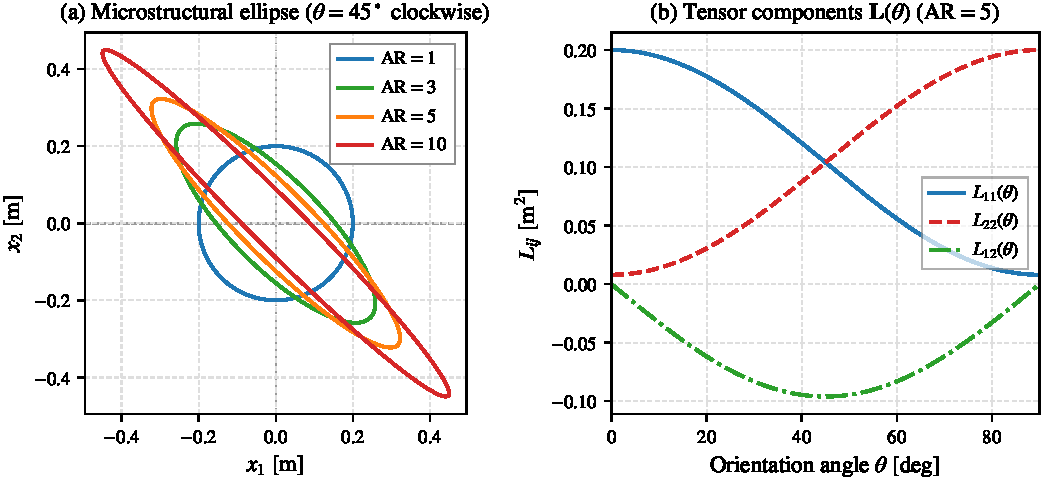
\includegraphics[width=\textwidth]{figures/fig01_ellipsoid_tensor.pdf}
\caption{(a) Volume-equivalent averaging ellipses at $\theta=45^\circ$ for $\mathrm{AR}=1,3,5,10$. (b) Length-tensor components versus orientation for $\mathrm{AR}=5$, including $L_{12}(45^\circ)=-0.096\,\mathrm{m}^2$ under the passive-rotation convention.}
\label{fig:ellipsoid_tensor}
\end{figure}

\subsection{Kinematics and constitutive response}
Assuming infinitesimal deformations under two-dimensional plane-strain conditions ($u_3 = 0, \partial(\cdot)/\partial x_3 = 0$), the classical displacement gradient and infinitesimal strain tensor $\bm\varepsilon$ are:
\begin{equation}
\varepsilon_{ij} = \frac{1}{2}(u_{i,j} + u_{j,i}), \quad i,j \in \{1, 2\}.
\label{eq:strain_def}
\end{equation}
In Mindlin's strain-gradient theory, the kinematic state includes the second displacement gradient or strain-gradient third-order tensor $\bm\eta$:
\begin{equation}
\eta_{ijk} = \varepsilon_{ij,k} = \frac{1}{2}(u_{i,jk} + u_{j,ik}), \quad \eta_{ijk} = \eta_{jik}.
\label{eq:strain_gradient_def}
\end{equation}
In 2D plane strain, the symmetric strain tensor $\bm\varepsilon$ contains 3 independent components ($\varepsilon_{11}, \varepsilon_{22}, 2\varepsilon_{12}$), while the strain-gradient tensor $\bm\eta$ possesses 6 independent components ($\eta_{111}, \eta_{112}, \eta_{221}, \eta_{222}, 2\eta_{121}, 2\eta_{122}$).

\paragraph{Mindlin Form-II constitutive law.}
We formulate the constitutive relations in Mindlin's Form II, wherein the strain energy density $W$ is decomposed into classical and higher-order strain-gradient contributions:
\begin{equation}
W = \frac{1}{2}\sigma_{ij}\varepsilon_{ij} + \frac{1}{2}\tau_{ijk}\eta_{ijk},
\label{eq:strain_energy_W}
\end{equation}
where $\bm\sigma$ is the Cauchy stress tensor and $\bm\tau$ is the third-order double-stress (or dipolar stress) tensor. For an isotropic base material parameterized by Lam\'e constants $\lambda$ and $\mu$, the Cauchy stress satisfies Hooke's law:
\begin{equation}
\sigma_{ij} = C_{ijkl}\varepsilon_{kl} = \lambda \delta_{ij}\varepsilon_{kk} + 2\mu \varepsilon_{ij}.
\label{eq:cauchy_stress}
\end{equation}
The double-stress tensor $\tau_{ijk}$ is conjugated to $\eta_{ijk}$ via an anisotropic gradient elasticity relation mediated by the characteristic-length tensor $\mathbf{L}$:
\begin{equation}
\tau_{ijk} = \frac{1}{10} L_{kl} C_{ijmn}\eta_{mnl} = \frac{1}{10} L_{kl}\left(\lambda \delta_{ij}\eta_{mml} + 2\mu \eta_{ijl}\right),
\label{eq:double_stress}
\end{equation}
where the prefactor $1/10$ arises from the second moment of the representative three-dimensional ellipsoidal averaging domain. Substituting Eq.~\eqref{eq:double_stress} into Eq.~\eqref{eq:strain_energy_W} demonstrates that $W$ is strictly non-negative and quadratic in both strains and strain gradients.

\paragraph{Gradient micro-inertia.}
To assess high-wavenumber regularization, the kinetic-energy density $T$ includes a gradient micro-inertia term:
\begin{equation}
T = \frac{1}{2}\rho \dot u_i \dot u_i + \frac{1}{2}\rho \ell_{\mathrm{i}}^2 \dot u_{i,j}\dot u_{i,j},
\label{eq:kinetic_energy_T}
\end{equation}
where $\rho$ is the macroscopic mass density and $\ell_{\mathrm{i}} > 0$ is the independent micro-inertia length parameter. Applying Hamilton's principle $\delta \int_{t_1}^{t_2} (T - W)\,\dif t = 0$ yields the strong-form equations of dynamic equilibrium in the bulk:
\begin{equation}
\sigma_{ij,j} - \tau_{ijk,jk} = \rho\left(\ddot u_i - \ell_{\mathrm{i}}^2 \ddot u_{i,jj}\right), \quad \text{in } \Omega.
\label{eq:strong_form}
\end{equation}
The Laplacian term $-\rho \ell_{\mathrm{i}}^2 \ddot u_{i,jj}$ on the right-hand side represents resistance to localized velocity gradients. For the shear branch examined here, Section~\ref{sec:steering} and Appendix~\ref{app:asymptotics} show that this term bounds the high-wavenumber phase speed.

\paragraph{Model reductions.}
The formulated anisotropic strain-gradient model contains four well-defined physical limits:
\begin{enumerate}[label=(\roman*)]
  \item \textbf{Classical Elasticity Limit ($l_m \to 0, \ell_{\mathrm{i}} \to 0$):} Double stresses vanish ($\tau_{ijk} \to 0$), micro-inertia vanishes, and the classical Navier equations of motion $\sigma_{ij,j} = \rho \ddot u_i$ are recovered with dispersionless acoustic speeds $c_T = \sqrt{\mu/\rho}$ and $c_L = \sqrt{(\lambda+2\mu)/\rho}$.
  \item \textbf{Isotropic Gradient Elasticity ($\mathrm{AR} = 1$):} Here $l_1 = l_2 = l_{\mathrm{iso}}$, so $L_{11} = L_{22} = l_{\mathrm{iso}}^2$ and $L_{12} = 0$ for all $\theta$, recovering isotropic Form-II gradient elasticity.
  \item \textbf{Gradient elasticity without micro-inertia ($\ell_{\mathrm{i}} = 0$):} Higher-order stiffness remains while dynamic regularization is removed; the transverse branch analyzed in Appendix~\ref{app:asymptotics} then has $v_p\propto k$ as $k\to\infty$.
  \item \textbf{Diagonal Rotation-Swap Symmetry ($\theta \to \theta + 90^\circ$ with $l_1 \leftrightarrow l_2$):} The components of $\mathbf{L}$ satisfy $L_{11}(\theta+90^\circ, l_1, l_2) = L_{22}(\theta, l_2, l_1)$ and $L_{12}(\theta+90^\circ, l_1, l_2) = -L_{12}(\theta, l_2, l_1)$, establishing rigorous rotational symmetry.
\end{enumerate}

\subsection{Boundary operators}
The variational formulation on boundary $\Gamma = \partial\Omega$ with unit outward normal $\bm n$ yields natural and essential boundary conditions:
\begin{equation}
p_i = \sigma_{ij}n_j - n_j n_k \tau_{ijk,k}, \quad R_i = n_j n_k \tau_{ijk},
\label{eq:traction_def}
\end{equation}
where $p_i$ is the effective surface traction and $R_i$ is the higher-order double traction. The corresponding work-conjugate kinematic variables are the displacement $u_i$ and the normal displacement derivative $\partial u_i/\partial n \equiv u_{i,j}n_j$.
